\documentclass[11pt,letterpaper]{article}
\usepackage[utf8]{inputenc} %Codificacion del texto (ISO Latin1 encoding)

\usepackage{fancyhdr} %Permite acomodar a tu gusto la parte de arriba y
% abajo del documento
\usepackage[spanish]{babel} %Permite definir el idioma del dcumento
\usepackage{graphicx} %Permite exportar imagenes en formato eps
\usepackage{url} %Tipo de fuente para correos y paginas
\usepackage{pgf}
\usepackage{fleqn}
\usepackage{amssymb}
\usepackage{fancyvrb}
\usepackage{sectsty}
\usepackage{makeidx}
\usepackage{colortbl} %Permite colocar colores a las tablas
\usepackage{booktabs}
%%%%%%%%%%
%Margenes%
%%%%%%%%%%
\parskip 1mm %Espacio entre parrafos

\setlength{\topmargin}{0pt}

\oddsidemargin	0.5cm  % Ancho Letter 21,59cm
\evensidemargin 0.5cm  % Alto  Letter 27,81cm
\textwidth	15.5cm
\textheight	21.0cm
\headsep	4 mm
\parindent	0.5cm
%%%%%%%%%%%%%%%%%%%%%%
%Estilo del documento%
%%%%%%%%%%%%%%%%%%%%%%
\pagestyle{fancyplain}

%%%%%%%%%%%%%%%%%%%%%%%%%%%%%%%%%%%%%%%%%%%
%Fancyheadings. Top y Bottom del documento%
%%%%%%%%%%%%%%%%%%%%%%%%%%%%%%%%%%%%%%%%%%%
% Recuerde que en este documento la portada del documento no posee
% numeracion, pero de igual manera llamaremos a esa primera pagina la numero
% 1, y la que viene la dos. Esto es para tener una idea de las que
% llamaremos pares e impares
\lhead{Sistemas y Organizaciones} %Parte superior izquierda
\rhead{\bf \it Informe 2} %Parte superior derecha
\lfoot{\it Análisis Organizacional} %Parte inferior izquierda. \thepage indica
% el numero de pagina
\cfoot{} %Parte inferior central
\rfoot{\bf \thepage} %Parte inferior derecha
\renewcommand{\footrulewidth}{0.4pt} %Linea de separacion inferior

% Challa

\newtheorem{theorem}{Theorem}
\newtheorem{acknowledgement}[theorem]{Acknowledgement}
\newtheorem{algorithm}[theorem]{Algorithm}
\newtheorem{axiom}[theorem]{Axiom}
\newtheorem{case}[theorem]{Case}
\newtheorem{claim}[theorem]{Claim}
\newtheorem{conclusion}[theorem]{Conclusion}
\newtheorem{condition}[theorem]{Condition}
\newtheorem{conjecture}[theorem]{Conjecture}
\newtheorem{corollary}[theorem]{Corollary}
\newtheorem{criterion}[theorem]{Criterion}
\newtheorem{definition}[theorem]{Definition}
\newtheorem{example}[theorem]{Example}
\newtheorem{exercise}[theorem]{Exercise}
\newtheorem{lemma}[theorem]{Lemma}
\newtheorem{notation}[theorem]{Notation}
\newtheorem{problem}[theorem]{Problem}
\newtheorem{proposition}[theorem]{Proposition}
\newtheorem{remark}[theorem]{Remark}
\newtheorem{solution}[theorem]{Solution}
\newtheorem{summary}[theorem]{Summary}
\newenvironment{proof}[1][Proof]{\noindent\textbf{#1.} }{\ \rule{0.5em}{0.5em}}

\newcommand{\primaria}[1]{
	\textbf{\underline{#1}}
}

\newcommand{\foranea}[1]{
	\textbf{\textsl{#1}}
}

\newcommand{\primyfor}[1]{
	\underline{\foranea{#1}}
}

\makeatletter
\newcommand\subsubsubsection{\@startsection {paragraph}{1}{\z@}%
                                   {-3.5ex \@plus -1ex \@minus -.2ex}%
                                   {1.5ex \@plus.2ex}%
                                   {\normalfont\bfseries}}
\newcommand\subsubsubsubsection{\@startsection {subparagraph}{1}{\z@}%
                                   {-3.5ex \@plus -1ex \@minus -.2ex}%
                                   {1.5ex \@plus.2ex}%
                                   {\normalfont\bfseries}}


\makeatother

%\makeindex
%%%%%%%%%%%%%%%%%%%%%%%%%%%%%%%%%%%%%%%%%%%%%%%%%%%%%%%%%%%%%%%%%%%
%%%%%%%%%%%%%%%%%%%% Aqui empieza el documento %%%%%%%%%%%%%%%%%%%%
%%%%%%%%%%%%%%%%%%%%%%%%%%%%%%%%%%%%%%%%%%%%%%%%%%%%%%%%%%%%%%%%%%%

\begin{document}

%%%%%%%%%%%%%%%%%%%%%%%%%%
%Definicion de la portada%
%%%%%%%%%%%%%%%%%%%%%%%%%%
\begin{titlepage}
    \begin{center}
	\begin{tabular}{ccc}
	     
\includegraphics[height=1.9cm]{images/utfsm}
	    & 
	    \hspace{0.2cm}
	    \begin{tabular}{c}
		Universidad Técnica Federico Santa María \\ \hline
		\hspace{8.0cm}
		\vspace{1.2cm}
	    \end{tabular}
	    \hspace{0.2cm}
	    &
            
\includegraphics[height=2cm]{images/di}
	\end{tabular}

	\vspace{1.5cm}
	%Titulo del Documento
	    \begin{tabular}{c}
		\Huge{\textbf{Informe 2}}\\\\
		\LARGE{\sc{Sistemas y Organizaciones}}\\
		\LARGE{\sc{{``Elian y Compañía''}}}
	    \end{tabular}

	\vspace{0.5cm}
	\begin{center}
		\Large{Teorías}\\
		\begin{itemize}
			\small
		        \item \textbf{Luther\ Gullick:} \emph{``PODSCORB''}\\
		        \item \textbf{Adam\ Smith:} \emph{``La Riqueza de las Naciones''}\\
		        \item \textbf{\'Emile\ Durkheim:} \emph{``Hechos sociales''}\\
		        \item \textbf{Frederick\ Taylor:} \emph{``Administración Científica''}
		        \item \textbf{Mary\ Parker\ Follet:} \emph{``El Nuevo Estado''}\\
		        \item \textbf{Chester\ Barnard:} \emph{``Influencia de factores sicológicos y sociales en la efectividad de la organización''}\\
		        \item \textbf{Fred\ Emery:} \emph{``Sistemas Sociotécnicos''}\\
		\end{itemize}

	\end{center}
	
        \vspace{1cm}

	%Nombre del (o los) autor(es)
	\begin{tabular}{cc}
	   \begin{tabular}{c}
         	\large{Rodrigo Fernández - 2673002-3}\\ 
		\large{\url{rfernand@inf.utfsm.cl}}\\
	   \end{tabular}
		&
	   \begin{tabular}{c}
         	\large{Javier Olivares - 2673043-0}\\ 
		\large{\url{jolivaro@inf.utfsm.cl}}
	   \end{tabular}
	\end{tabular}
	   \begin{tabular}{c}
		\\
         	\large{Cristi\'an Maureira - 2673030-9}\\ 
		\large{\url{cmaureir@inf.utfsm.cl}}\\
	   \end{tabular}

	% Nombre profesor asignatura
	\begin{center}
		\large{\textbf{Profesor:} Lautaro Guerra Genskowsky}
	\end{center}

        \vspace{1cm}
	%Fecha
		\large{\sc{\today}}
    \end{center}
\end{titlepage}

\newpage

\tableofcontents
\newpage

\section{Resumen}
\label{sec:resumen}
%Explicar el contenido del trabajo en unas pocas líneas.

%Hablar de la empresa, dar como una introduccion
%seria ideal poner la informacion que tenemos de cuando hablamos con mauricio,
%la primera vez que fuimos

Este trabajo consiste en un análisis organizacional desde el punto de vista de 7 teorías, muy importantes
para el estudio de las organizaciones, de la micro-empresa ``Elian Y Cía., Ltda.''.

Esta micro-empresa se encarga de la producción, venta y reparaciones de joyas, lleva más de veinte años en
la Quinta Región. Dispone de talleres propios siguiendo procesos a cargo de orfebres especializados.
Elaboran todo tipo de cadenas, anillos, argollas de matrimonio y colgantes (de oro y plata).
Se han preocupado por implementar nuevas tecnologías, ofreciendo fotograbado a color en Plata, Oro y
Acero.

Posee 4 sucursales de ventas y una casa central donde tienen todo el proceso de producción. El personal
no son más de 30 personas, es una organización exigente, pero preocupada por el bienestar de sus
trabajadores. Como se manejan objetos pequeños de gran valor, la confianza en los trabajadores y buenos
métodos de control son primordiales para la empresa. Por ello, el ambiente entre los colaboradores es muy
familiar, donde la alta gerencia está conformada por el jefe de todos, Sr. Iván González y el gerente de
ventas y producción, su hijo Iván González.

Las áreas de trabajo en la empresa se pueden identificar como
ventas (vendedores de cada sucursal), producción (la mayoría orfebres) y administración (secretarias, 
informática y gerencia).

\newpage

\section{Antecedentes}
\label{sec:antecedentes}
%Investigación de las teorías a aplicar en la organización (cada una debe estar bien detallada).
%(No está permitido el copy/paste de las ppt del ramo).

\begin{itemize}
	\item \textbf{Luther\ Gullick:} \emph{``PODSCORB''}\\
	% Lista
	Basándose en el estudio de Fayol,
	postula apuntes de la Ciencia de Administracion (junto a Urwick),
	donde postula los 7 principios que un gerente debe realizar,
	``PODSCORB'',
	Además cabe mencionar que fue la teoría más importante del autor,
	la cual resumió en una sola palabra compuesta por las iniciales de cada uno de los siete principios:
	\begin{itemize}
		\item Planificación
		\item Organización
		\item Dirección
		\item Formación del plantel(Staffing)
		\item Coordinación
		\item Reporte
		\item Presupuestar
	\end{itemize}
	Gullick agrega nuevos elementos al proceso de la Administración,
	como lo es en el caso del ``Estado Benefactor'',
	ya que la crísis vivida en ese momento,
	requería mayor eficiencia en la ayuda que se daba en cuanto a demandas sociales,
	seguridad, alimentación, vivienda, entre otras.
	
	Por lo tanto,
	se dice que existe un estado benefactor cuando el estado asegura protección social.

	\item \textbf{Adam\ Smith:} \emph{``La Riqueza de las Naciones''}\\
	% Listo
	Adam Smith es el Padre de la economía moderna (capitalismo),
	en la teoría anteriormente señalada,
	Smith intentó diferenciar la Economía Política de la Ciencia Política,
	la ética y jurisprudencia.
	
	En ésta teoría critica al mercantilismo;
	búsqueda de un orden económico que funcionara mejor no tomando en cuenta el estado.

	Plantea también que la clave del bienestar social,
	está en el crecimiento económico y se potencia por la división del trabajo.

	``Gracias a la apelacion al Egoísmo se logra el bienestar General''

	Recordemos que en el Mercantilismo,
	el sistema se basa en la propiedad privada y
	en la utilización de los mercados como forma de organizar la actividad económica.
	es decir, maximizar el interés del Estado soberano y no de los propietarios.
	Lo cual era totalmente lo contrario del Capitalismo de Smith.
	
	Finalmente,
	Smith plantea dos ideas claves,
	para poder seguir el camino del Capitalismo:
	Explicar los factores que determinan el progreso económico y
	las medidas que podrían tomarse para crear ambiente favorable para el crecimiento económico y
	que los ingresos per capita se deben a la destreza de cada persona.
		
	\item \textbf{\'Emile Durkheim:} \emph{``Hechos sociales''}\\
	% Listo
	Es el Padre de la sociología;
	durante su vida planteó variadas ideas,
	como la del ``Trabajo Social'' y la idea de los ``Hechos sociales'',
	ésta última es la que se utilizará en nuestro trabajo y también
	es considerada la más importante.

	Primero que todo,
	debemos notar que  ``Los Hechos Sociales'' separaron la sociología de la sicología,
	señalando que todo lo que ocurría a nuestro alrededor,
	era un hecho social y poseía las siguientes características:
	\begin{itemize}
			\item Exterioridad, ocurren fuera de nuestra persona.
			\item Coerción, poseen cierta influencia sobre nosotros.
			\item Colectividad, no sólo nos ocurren a nosotros, sino a todos nuestros similares.
	\end{itemize}

	Los hechos sociales tienen otra condición no menos importante que las anteriores,
	y que es la de encarnarse en la psiquis de cada individuo de una sociedad
	y por tanto transformar la forma subjetiva de sentir determinados hechos o situaciones,
	por esta misma razón adquieren un carácter sui géneris,
	con valor en sí mismo y no como resultado de otros hechos sociales.
	
	Esta forma de sentir cuando el hecho se presenta frente a la presencia de un grupo puede dar
	lugar a otro fenómeno social, que Durkheim determina ``Corrientes Sociales''.

	Finalmente,
	lo que debemos comprender acá,
	es que según Durkheim
	todo hecho que ocurre a nuestro alrededor,
	es un hecho social (con las características anteriormente señaladas),
	es decir,
	la sociedad es lo más importante,
	y rige nuestro actuar, nuestro pensar, todo.
	
	\item \textbf{Frederick\ Taylor:} \emph{``Administración Científica''}
	
	La Administracion Científica de Taylor,
	aborda aspectos como estudios de tiempos y movimientos,
	selección de obreros,
	métodos de trabajo,
	incentivos,
	especialización e
	instrucción.

	La idea principal es optimizar la manera que el trabajo es realizado
	y simplificando el trabajo realizado por los trabajadores,
	para que fueran capacitados
	sólo para realizar esta función de la mejor forma posible.

	Esta teoría quitó esta autonomía y
	el trabajo que sólo un experimentado artesano
	ahora será realizado por trabajadores que tienen asignada una tarea simple de realizar
	y que es fácil de aprender. 

	Taylor identifica los males principales en una organización:
	\begin{itemize}
		\item Holgazanería por parte de los trabajadores. 
		\item Falta de información por parte de la Administración hacia los obreros.
		\item Falta de técnicas de trabajadores. 
	\end{itemize}

	Finalmente,
	Taylor al presentar su teoría se basa en los siguientes fundamentos:
	\begin{itemize}
		\item Desarrollar para cada elemento del trabajo del obrero,
			una ciencia que reemplaza los antiguos métodos empíricos. 
		\item Selecciona científicamente y luego instruye,
			enseña y forma al obrero de acuerdo con sus propias posibilidades. 
		\item Coopera cordialmente con los obreros,
			para que todo el trabajo sea hecho
			de acuerdo con los principios científicos que se aplican.
		\item Distribuye equitativamente el trabajo y
			la responsabilidad entre la administración y los obreros. 
	\end{itemize}

	\item \textbf{Mary\ Parker\ Follet:} \emph{``El Nuevo Estado''}\\
	% Listo
	Follet es una de las creadoras de los inicios básicos de la Administración.
	Su estudio sobresalió porque sostenía la existencia
	de principios generales,
	que eran aplicables en \emph{todas} las organizaciones.

	A través de su vida,
	defendio el principio de lo que ella llamó como \emph{``integración''};
	el ``poder con'' en vez del ``poder sobre''.
	
	Principalmente,
	la enseñanza que Follet nos deja,
	y que será utilizada en el análisis de ésta organización,
	es que los Jefes no deben tratar como cualquier cosa a los trabajadores,
	sino que cada trabajador es una persona y tiene sus derechos,
	por lo que deben sentirse parte de la organización,
	con buenos tratos.

	``Sólo podremos encontrar al verdadero hombre en la organizacion de grupo.''
	
	\item \textbf{Chester\ Barnard:} \emph{``Influencia de factores sicológicos y sociales en la efectividad de la organización''}\\
	% Listo
	Barnard nos entrega un esquema conceptual
	de la teoría de las organizaciones basado en:
	\begin{itemize}
		\item Racionalidad individual y grupal.
		\item Cooperación.
		\item Organizacion Formal e Informal.
	\end{itemize}

	Además el define la Organizacion, 
	como un sistema de actividades o fuerzas,
	conscientemente coordinadas de 2 o más personas.

	Otros puntos importantes en su estudio,
	es que avalaba el hecho de que los trabajadores de una organización,
	poseían limitaciones físicas y biológicas que los obligan a trabajar en grupo.
	Por lo cual la cooperación es fundamental en una organización.

	Su teoría ha servido para ir un paso mas allá
	en la Administración Científica y en los principios de Fayol.

	Finalmente,
	Barnard nos enseña que mantener una organización en un correcto funcionamiento implica:
	\begin{itemize}	
		\item Esforzarse para mantener la comunicación organizacional.
		\item Asegurar los servicios escenciales para los trabajadores.
		\item Formulación del ``propósito'' y de los objetivos.
	\end{itemize}

	\item \textbf{Fred\ Emery:} \emph{ ``Sistemas Sociotécnicos''}\\
	
	Emery nos plantea la teoría de los Sistemas Sociotécnicos
	en el ``Desarrollo Organizacional'',
	lo cual implica un esfuerzo planificado en toda la organización
	y controlada desde el nivel más alto de efectividad.

	A través de experimentos,
	logró darse cuenta que la tecnología sóla no funciona,
	por eso es necesario un sistema sociotécnico.

	Lo anterior se debe a que los trabajadores,
	al ver tecnología en la organización,
	se relaja, y comienza a haber mucho absentismo,
	además de haber ciertas disputas por lo mismo,
	crea un ambiente individualista y los trabajadores
	no se sienten parte de la empresa.

	Finalmente,
	el punto crucial en ésta teoría
	es que Emery se da cuenta que el sistema Tayloriano,
	es erróneo, por lo cual debemos hacer el trabajo
	en equipos, lo cual aparte de aumentar la productividad
	implica una cierta satisfacción personal,
	ya que se mejora mucho el ambiente de trabajo.
	
\end{itemize}

\newpage

\section{Desarrollo}
\label{sec:desarrollo}
\subsection{Memoria Principal y Memoria Caché}

	En la primera parte de ésta serie de papers, logramos ver que 
las operaciones aritméticas más comunes, toman entre 1 a 10 ciclos de 
CPU. Sin embargo, para poder realizar estas operaciones, es necesario
 contar con el medio de almacenamiento necesario para los datos utilizados
 en cada operación, por lo que se hace primordial, tener en consideración 
el acceso a este medio. El acceso a la memoria principal puede tomar
 aproximadamente unos 300 ciclos de CPU, por lo que si se desarrollan 
algoritmos optimizados, todo el esfuerzo es en vano si el acceso a la 
memoria principal produce grandes latencias.\\\\
	Para suerte de nosotros, los diseñadores de hardware han desarrollado
 estrategias para cubrir este gran problema, para ello decidieron colocar una
 pequeña memoria en una posición muy cercana al CPU, a la cual denominan memoria
 caché, las cuales poseen una característica importante, ser extremadamente 
rápida. Con esta disposición, los datos son accesados mucho mas rápida que si
 fueran leídos desde la memoria principal. Los procesadores más modernos poseen 
dos o más niveles de caché, denominados L1,L2 y así sucesivamente, los que dan 
a tranzar entre tamaño y velocidad. Leer desde la memoria cache L1 es muy rápido
 comparado con la memoria principal, pero a su vez tiene mucha menos capacidad 
de almacenamiento.\\\\
	La principal tarea de los programadores, es entonces, lograr un 
entendimiento sólido en este aspecto, para de esta forma llegar a comprender
 en que condiciones los datos son almacenados en la memoria caché y así lograr
 asegurar que los datos que necesitemos, se encuentren en ella.

\subsection{Localidad}

Primero que todo debemos comprender que el cache funciona \emph{reteniendo los datos utilizados recientemente},
para poder obtenerlos mas rápido en una próxima situación.
Obviamente no es posible retener los datos por un tiempo indefinido,
por lo cual son retenidos el máximo tiempo posible y van a salir de la memoria cache,
solo cuando otros datos necesiten ser retenidos.

Por lo tanto el paper analizado nos plantea que una forma de reducir la frecuencia de tener que ir a la memoria principal en variadas ocasiones,
es reutilizar los datos todas las veces que sea posible posible dentro de un periodo de tiempo corto,
porque los datos seguirán estando en el cache y no tendremos que hacer todo el procedimiento de nuevo

El concepto anteriormente señalado es conocido como \emph{localidad temporal}

Como hablamos de \emph{localidad temporal},
también es necesario tocar el tema de la \emph{localidad espacial},
la cual corresponde a cuando un programa usa múltiples partes de datos que han sido guardados contiguos en un periodo corto de tiempo.
El ejemplo que el paper ilustra de localidad espacial,
facilita la comprensión, éste nos señala una simple situación de recorrer un arreglo secuencialmente.

Por otro lado el cache aprovecha la \emph{localidad espacial} recuperando y almacenando toda la secuencia de bytes contiguos,
es decir, no sólo los bytes específicos de los datos solicitados por el procesador.
\emph{¿Cuál es la idea de recuperar y almacenar toda la secuencia de bytes?}
Claramente es poder satisfacer futuras solicitudes de direcciones de memoria cercana.

Hay otra forma en la cual una \emph{localidad espacial} de programas puede mejorar el desempeño del cache,
esta se basa en aspecto del funcionamiento del cache.
Si todo fuera perfecto cualquier linea de datos podría estar en una linea de cache,
pero para poder limitar el numero de lineas que deben ser buscadas y poder conservar los tiempos de acceso al cache cortos,
el mismo cache se preocupa de limitar las lineas de cache donde pueden estar las lineas de datos.

\begin{center}
	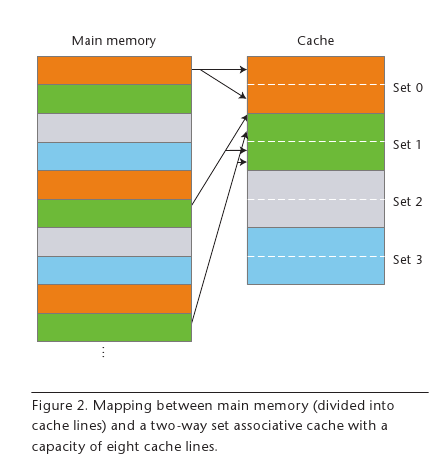
\includegraphics[scale=0.7]{images/figura2}
\end{center}

Las áreas verdes en la memoria principal pueden mapear solo una de dos lineas de cache verdes en el cache.
Si mas de dos áreas mapean el mismo conjunto,
resulta un conflicto, causando que algunos datos sean desalojados.

El conflicto de que dos áreas mapeen el mismo conjunto puede ser evitado con ayuda de la \emph{localidad espacial},
porque áreas contiguas en la memoria principal garantizan un mapeo a diferentes conjuntos en el cache.

\subsection{Mejorando la localidad espacial: \emph{Array-Merging}}
Esta Técnica, \emph{Array-Merging}, se utiliza para mejorar el tiempo de acceso a los datos en la \emph{memoria principal}.
En el ejemplo, se declaran los siguientes arreglos:
\begin{lstlisting}[language=C]
 int x[N], y[N];
 float sin6[N], cos6[N];
 int count[MAX_R];
 float g[MAX_R];
\end{lstlisting}

\begin{center}
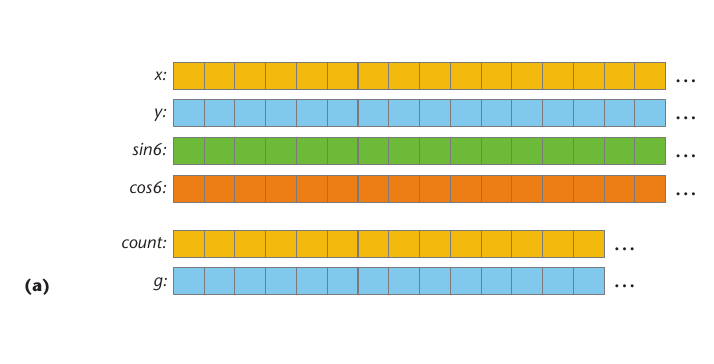
\includegraphics[scale=0.6]{images/array-1.png}
\end{center}

Si bien esto mejora el tiempo de acceso a los datos, solo sirve para requerimientos de los arreglos, ya sea $x[N]$ o $y[N]$, pero en el programa necesitamos acceso a el elemento \emph{n-esimo} de los 4 arreglos de input y el elemento \emph{r-esimo} de los 2 arreglos de output al mismo tiempo. Para mejorar la localidad espacial usamos el método del que hablamos, \emph{Array-Merging}, que guarda los valores, asociado a cada \emph{n-esimo} elemento, de forma contigua. 
Para poder llevar a cabo esta técnica podemos utilizar C, donde debemos definir estructuras donde poner cada uno de nuestros arreglos. Con esto cada vez que la memoria Cache necesite los valores, de manera anexa, también guardara los demás valores que serán necesarios. Esto lo podemos ver en el siguiente código.

\begin{lstlisting}[language=C]
struct DataStruct {
 int x, y;
 float cos6, sin6; };
DataStruct data[N];
struct AccumulationStruct {
 int count;
 float g; };
AccumulationStruct accum[Max_R];

//Now, accumulate data for all pairs of
//points (i,j).
for(i=0; i<N; ++i) //for each i < N
 for(j=i+1; j<N; ++j) { //for each j < N
  Dx = data[i].x - data[j].x;
  Dy = data[i].y - data[j].y;
  r = sqrt(Dx*Dx + Dy*Dy);
  accum[r].g += data[i].cos6 * data[j].cos6 +
   data[i].sin6 * data[j].sin6;
  ++accum[r].count;
}
\end{lstlisting}


\begin{center}
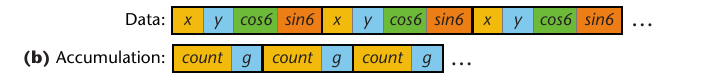
\includegraphics[scale=0.6]{images/array-2.png}
\end{center}

\subsection{Mejorando la localidad temporal: \emph{Blocking}}

La idea de mejorar la localidad temporal, es la de mantener los datos más recientemente accedidos
``cercanos'' al procesador.

El método consiste en agrupar las variables de entrada en pequeños bloques (del tamaño
\emph{blocksize}) que quepa fácilmente en el cache de menor nivel. Entonces, podemos procesar cada
par posible de puntos de esos dos bloques antes de pasar a procesar el siguiente par de bloques.
% como muestra la figura 4(...).
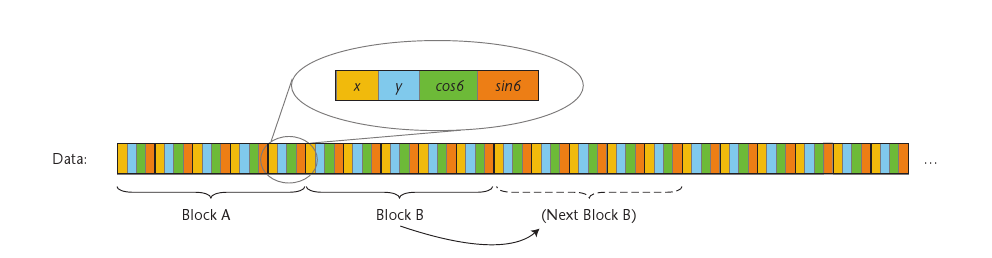
\includegraphics[scale=0.7]{images/figure4}

De esta forma, se logran realizar más computaciones por cada nuevo punto de información leído de la
memoria principal. Por ejemplo, si guardamos en el caché dos bloques de información, cada uno con un
tamaño de 100 puntos, podríamos procesar todos los 10.000 pares de puntos posibles antes de tener que
acceder al siguiente bloque de 100 puntos, lo cual es una gran mejora comparada con procesar un solo par
de puntos por cada punto leído.

La porción de código modificado queda como sigue:\\
\scriptsize
\begin{lstlisting}[language=C]
for(A = 0; A+2*blocksize < N; A+= blocksize)
	for(B=A+blocksize; B+blocksize<N; B+=blocksize)
		for(i=A; i<A+blocksize; ++i)
			for(j=B; j<B+blocksize; ++j)
			{
				(...)
			}
(...)
\end{lstlisting}
\normalsize
La desventaja de esta técnica consiste en que el código se vuelve más complejo y necesita la
implementación de más código para le manejo de nuevos casos especiales (rangos fuera de índices y evitar
que falten o se repitan operaciones).\\
 Si vemos el código, nos damos cuenta que aumentamos el número de iteraciones anidadas de 2 a 4.
Además, este no incluye los casos especiales para que funcione.\\

Por ello, nos vimos obligados a implementar nuestro própio código para probar el método de ``blocking''
en el algoritmo:
\scriptsize
\begin{lstlisting}[language=C]
	for(A=0; A<N; A+=blocksize)
	{
		C=A;
		for(B=A,flag=1; B<N; B+=blocksize,flag=0)
		{
			for(i=A; i<A+blocksize; ++i)
			{	
				if(flag)
				{
					C++;
					for(j=C; j<B+blocksize; ++j)
					{
						(...)
					}
				}
				else
					for(j=B; j<B+blocksize; ++j)
					{
						(...)
					}
			}
			C=B;
		}
	}
(...)
\end{lstlisting}
\normalsize


\textbf{Resultados}\\
En los casos de prueba  aumentó el tiempo de procesamiento en comparación con el código original.\\
Posibles causas de este resultado:
\begin{itemize}
        \item Nuestro hardware ya estaba haciendo un excelente trabajo.
        \item El aumento de operaciones por cada ciclo no se compensaba
\end{itemize}

Para más información del código utilizado, ver los anexos.

\subsection{Mejoras propuestas en nuestra investigación}
\subsubsection{Aproximación de raíces}

Utilizaremos una \emph{lookup table}, la cual es una estructura de datos, usualmente un arreglo o un arreglo asociativo.
Esta tabla es usada para reemplazar un cálculo en tiempo de ejecución,
con una simple operación de indexación de un arreglo.

Por lo tanto nos remontamos al siguiente \emph{código}:

\textbf{Original}
\begin{center}
\begin{lstlisting}[language=C]
...
for(j=i+1;j<N;++j)
{
	Dx = data[i].x - data[j].x;
	Dy = data[i].y - data[j].y;
	r = sqrt(Dx*Dx + Dy*Dy);
	accum[r].g+=data[i].cos6 + data[j].cos6 +data[i].sin6 + data[j].sin6;
	++accum[r].count;
}
...
\end{lstlisting}
\end{center}
\textbf{Modificado}
\begin{center}
\begin{lstlisting}[language=C]
...
for(j=i+1;j<N;++j)
{
	Dx = data[i].x - data[j].x;
	Dy = data[i].y - data[j].y;
	root(Dx*Dx + Dy*Dy, r)
	accum[r].g+=data[i].cos6 + data[j].cos6 +data[i].sin6 + data[j].sin6;
	++accum[r].count;
}
...
\end{lstlisting}
\end{center}

Nuestra función \emph{root()} la hemos implementado aparte en un archivo \emph{.h};
el cual no es nada más que un \emph{switch} con muchos \emph{case}.

\begin{center}
\begin{lstlisting}[language=C]
#define root(x,y)
	switch(x){
	case 0: y = 0; break;
	case 1: y = 1; break;
	case 2: y = 1; break;
	case 3: y = 1; break;
	...
	case 997: y = 31; break;
	case 998: y = 31; break;
	case 999: y = 31; break;
	}
\end{lstlisting}
\end{center}

Lo cual nos sirve para poder acceder a \emph{aproximaciones} de valores,
en vez de tener que calcular la raíz de un determinado numero.

Obviamente en la vida real,
se utilizan tablas mucho mas grandes.


\subsubsection{Aproximación de funciones trigonométricas}
Como en nuestro código realizamos muchos cálculos de \emph{funciones trigonométricas},
tenemos como motivación poder optimizar el tiempo y cálculo de éstas.

Podemos recordar las \emph{Series de Taylor}, para realizar una suerte de aproximación.

$$\sin{x} = \sum^{\infty}_{n=0} \frac{(-1)^n}{(2n+1)!} x^{2n+1} = x - \frac{x^3}{3!} + \frac{x^5}{5!} - \ldots \forall x$$

El problema radica en que algunos computadores, no pueden calcular el \emph{seno} de un valor dado,
pues están limitados a realizar operaciones básicas.

Las series de Taylor nos brindan una herramienta para poder calcular ciertas funciones trigonométricas,
con una gran presición.

Ocuparemos entonces una aproximación para calcular el \emph{seno}:

$$\sin{x} \approx x - \frac{x^3}{6} + \frac{x^5}{120} - \frac{x^7}{5040}$$

Pero, ocupamos muchas multiplicaciones para calcular los $x^k$,
por lo cual utilizaremos el \emph{Algoritmo de Horner}.

Éste algoritmo plantea una forma de calcular eficientemente polinomios de una forma monomial,
es decir,
$$ p(x) = a_0 + a_1 x + a_2 x^2 + a_3 x^3 + \cdots + a_n x^n $$

Por lo tanto podremos reducir nuestro polinomio:
$$\operatorname{sin}(x) \approx x - \frac{x^3}{6} + \frac{x^5}{120} - \frac{x^7}{5040}$$
		a,
$$\operatorname{sin}(x) \approx x \left( 1 - x^{2}\left(\frac{1}{6} + x^{2}\left(\frac{1}{120} - \frac{x^2}{5040}\right)\right)\right)$$

Si nos damos cuenta estamos reduciendo el número de multiplicaciones de 12 a 3

Luego de varias pruebas en el cálculo de efectuar ésta operación,
nos dimos cuenta que se transforma en un cálculo muy caro,
especialmente para procesadores lentos.

\subsection{Pruebas}
\subsubsection{Justificación}

Actualmente casi todos contamos con computadores con una capacidad respetable en comparación a las últimas tecnologías existentes,
pero estamos descuidando un área muy popular, los cuales son los sistemas embebidos.

Es por eso que en nuestro trabajo hemos optado por trabajar con un equipo con arquitectura ARM\footnote{http://es.wikipedia.org/wiki/ARM},
pues su capacidad de procesamiento es mucho menor, pero aspira alcanzar procesamientos al mismo nivel que un computador normal.
Si nos damos cuenta, la mayoría de los dispositivos como celulares, pocketpc, netbooks, etc, poseen poca memoria y necesitan que cada operación que se realice
sobre ella sea lo más óptima posible.

Finalmente,
una mejora en un algoritmo en un computador de escritorio o notebook actual, quizás no podremos notar la diferencia,
pero en sistemas embebidos pueden significar un gran ahorro de tiempo y provocar un mayor desempeño.

\subsubsection{Hardware}

	El kit de desarrollo Intrinsyc's Cerf$^{TM}$Board 250 provee una plataforma 
flexible, con hardware y software de alto desempe\~no para desarrollar aplicaciones 
embebidas en forma r\'apida. El kit incluye:

\begin{itemize}
	\item Intel PXA250 (XScale)
	\item Tarjeta de expansi\'on Cerf IO 250
	\item Tarjeta de expansi\'on CerfComm 250
	\item Intrinsyc's I-Linux con kernel 2.4
\end{itemize}

\begin{center}
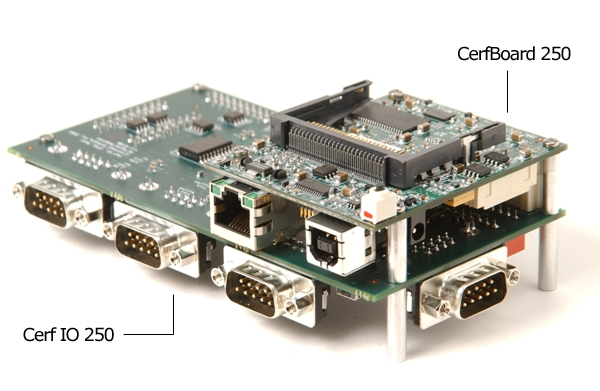
\includegraphics[scale=0.3]{images/board}
\end{center}

\subsubsection{Intel PXA250 (XScale)}

	El Intel PXA250 es un microprocesador basado en un n\'ucleo Intel XScale.
Intel XScale es una micro arquitectura RISC de 32-bit basado en una arquitectura ARM. Dise\~nado para un alto desempe\~no a costa de usar poca energ\'ia. Incorpora un conjunto completo de sistemas y perif\'ericos, funciones que le permite ser utilizado en una variedad de port\'atiles de mano.

	Posee las siguientes caracter\'isticas t\'ecnicas:

\begin{itemize}
	\item Frecuencia de 400MHz
	\item Memoria Principal de 64MB
	\item Cach\'e de instrucciones de 32KB
	\item Cach\'e de datos de 32KB
	\item B\'ufer de 256 bit
	\item Controlador de memoria basado en una arquitectura de memoria unificada, donde todos los dispositivos de memoria externos comparten un bus de direcci\'on y datos en com\'un.
	\item El controlador de memoria consiste en cuatro unidades de control principal para dar interfaz a memorias din\'amicas (SDRAM), memorias est\'aticas (ROM, SRAM, Flash), PCMCIA y chips similares.
	\item La memoria externa es vista como una colecci\'on lineal de bytes numerados desde 0 hacia adelante.
\end{itemize}

\begin{center}
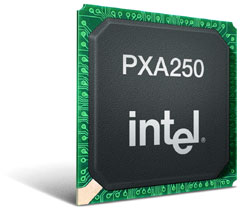
\includegraphics[scale=0.5]{images/pxa250}
\end{center}

\subsubsection{Tarjeta de expansi\'on Cerf IO 250}

	La tarjeta de expansi\'on Cerf IO 250 es una placa con entrada y salida
de propósito general. Viene equipada con un puerto serial de depuraci\'on RS232,
dos puertos seriales RS232, un puerto serial RS422/485, entre otros.

\subsubsection{Tarjeta de expansi\'on CerfComm 250}

	La tarjeta de expansi\'on CerfComm 250 est\'a equipada con caracter\'isticas
en la comunicaci\'on, viene con un controlador USB Host, un puerto Ethernet  10/100
 y tres puertos seriales de depuraci\'on RS232.

\subsubsection{Resultados}

	Para la realización de las pruebas consideramos una cantidad de datos 
igual a 50000, por otro lado programamos dos ejemplos, el primero de ellos consiste 
en la implementación mas rápida de codificar, sugerida por los papers, mientras 
que el segundo ejemplo incluye las optimizaciones sugeridas,
a continuación los resultados:\\

\begin{tabular}{|l|l|l|l|l|}
\hline
& Normal & Optimización 1 & Optimización 2 & Optimización 3 \\
\hline
Tiempo ejecución [s] & 143 & 55 & 54 & 54\\
\hline
\end{tabular}

\begin{itemize}
	\item Optimización 1: Calculo previo de funciones trigonométricas
	\item Optimización 2: Array merging
	\item Optimización 3: Blocking
\end{itemize}



\newpage

\section{Conclusiones individuales}
\label{sec:conclusionesIndividuales}
%Cada alumno se identifica y da una conclusi?n personal acerca de los temas tratados.

\begin{itemize}
	\item Javier Olivares

		Sin duda la organización se caracteriza por su complejidad y variedad, a pesar de esto no ha sido 
		complicado encontrar ciertos parámetros y situaciones que se acercan a las propuestas por los 
		distintos pensadores revisados en el ramo y particularmente a los analizados en este informe. 
		Este trabajo me ha sido de gran ayuda para entender como se estructura una organización, y además como 
		deben ser las interacciones entre las personas y herramientas que la componen. 
		
		Otra importante conclusión es que la empresa trabaja cumpliendo con varios postulados de los autores, pero
		sin tener quizás clara conciencia de esto, lo cual valida mayormente todas las teorías y postulados 
		propuestos por los pensadores mostrándonos que a pesar del paso del tiempo todas estas siguen siendo 
		válidas y estrechamente relacionadas con la realidad del día a día de la organización.
		
		Gracias al apoyo entregado por la jefatura de la empresa, hemos podido entrevistar a trabajadores de
		distintas áreas obteniendo respuestas sinceras, logrando una mirada global uniendo las ideas de cada uno de
		los trabajadores y jefes.

	\item Rodrigo Fernández

		Es muy importante mantener un ambiente de unidad dentro de los diferentes grupos de cada organización,
		preocupándose del bienestar de los trabajadores para que se sientan acogidos y atendidos mientras
		realizan su trabajo. De esta forma, se motiva a los trabajadores por mantener ese ambiente y acogen más
		facilmente las metas y objetivos comunes de la empresa.

		Además, el otorgarles no sólo el bienestar económico, sino las libertades necesarias para que puedan
		desarrollar su personalidad y fraternizar con sus co-trabajadores, ayuda a generar mejores equipo de
		trabajo y a generar una organización orgánica.

	\item Cristián Maureira
	
		Cuando uno habla de organización, no nos damos cuenta de la importancia de tal.
		Una organización es mucho más que un Jefe con Empleados, que desarrollan una cierta actividad,
		una organización es un ser, formado por cada trabajador de ella, sin importar su cargo,
		todos son partes fundamentables, es por eso que cuando uno se refiere a la idea de organización
		estamos hablando de un conjunto de personas que tienen un mismo objetivo en común.

		Es necesario sentirse identificado con el lugar donde uno trabaja,
		por el simple hecho que el trabajo se hace mucho más agradable, y nos volvemos más
		productivos; lo que beneficia a la organización y a mi mismo.

		El trabajo realizado, nos sirvió para comprender que hacer una \emph{teoría}
		acerca de mecanismos de trabajos, o de como debe ser una organización,
		es una tarea compleja, que requiere un estudio minuciosos, a la misma organización
		ya que es necesario poder saber la impresión de cada trabajador,
		saber si las normas son correctas o no,
		darnos cuenta si la productividad aumenta o disminuye con ciertos cambios en el ambiente laboral, etc.

		Un punto importante que me gustaría recalcar,
		es el hecho de que se trataba de una organización no muy grande,
		lo que creaba un ambiente grato, pues todos se conocian mutuamente,
		y más que compañeros de trabajo, habían muchos lazos de amistad;
		lo cual es completamente positivo, por el hecho de que es mas agradable nuestro día a día.
		Al ser pequeña, también facilitaba la comunicación con compañeros de trabajo y con el mismo jefe,
		lo que nos dió a entender, que todos los trabajadores son escuchados,
		y que cada persona relacionada con la organización tiene su grado de importancia.


\end{itemize}


\newpage

\section{Conclusiones generales}
\label{sec:conclusionesGenerales}
%Conclusión elaborada por todos los miembros del equipo en conjunto.

Esta actividad nos ha permitido entender de manera sistémica el funcionamiento de una organización,
ya que si bien se analizó sólo una cantidad limitada de integrantes, es posible obtener un 
esquema relativamente claro de como se estructura el sistema, en este caso la organización 
analizada, de como interactúan sus partes, es decir los trabajadores y jefes, y además de como la 
organización se relaciona con el ambiente.

Es fácil encontrar, en este caso, una relación entre las respuestas de cada uno de los entrevistados
teniendo una opinión común de la organización en la que están insertos. Esto nos indica
la existencia de una organización estable, con objetivos captados claramente por todos los integrantes. Si
bien existen ciertos puntos de vista que varían según el entrevistado, no se alejan completamente del
pensamiento global.

\newpage

\section{Bibliografía}
\label{sec:bibliografia}
% daa!
\begin{itemize}
	\item Web de la Empresa, \emph{http://www.ivangonzalezjoyas.cl}
	\item \emph{http://es.wikipedia.org/wiki/Hecho\_social}
	\item \emph{http://en.wikipedia.org/wiki/Luther\_Gulick\_(social\_scientist)}
	\item \emph{http://es.wikipedia.org/wiki/La\_riqueza\_de\_las\_naciones}
	\item \emph{http://es.wikipedia.org/wiki/Administraciíon\_Científica}
	\item \emph{http://sunsite.utk.edu/FINS/Mary\_Parker\_Follett/Fins-MPF-01.html}
	\item \emph{http://en.wikipedia.org/wiki/Chester\_Barnard}
	\item \emph{http://es.wikipedia.org/wiki/Sistema\_socio-técnico}
\end{itemize}

\newpage

\section{Anexos}
\label{sec:anexos}
\scriptsize
\subsection{C\'odigo base}
\begin{verbatimtab}
#include <math.h>
#include <stdlib.h>
#include <stdio.h>
#include "global.h"

int x[N], y[N];
float theta[N];
int count[N];
float g[(int)(N*1.5)];

int main(int argc, char **argv)
{
	for(i=0;i<N;i++)
	{
		x[i] = i;
		y[i] = i;
		theta[i] = 6*random();
	}

	//	Almacenamos tiempo capturado
	initialTime = getTime();

	//	Now, accumulate data for all pairs of
	//	points (i,j).
	for(i=0; i<N; ++i)	//for each i < N
		for(j=i+1; j<N; ++j)	//for each j < N
		{
			Dx = x[i]-x[j];
			Dy = y[i]-y[j];
			r = sqrt(Dx*Dx + Dy*Dy);
			g[r] += cos(6*(theta[i]-theta[j]));
			++count[r];
		}

	for (r = 0; r < MAX_R; r++)
		g[r] = g[r] / count[r];

	//	Calculando lo que ha tomado el calculo
	finalTime = getTime();

	//	Imprimimos resultados
	results();
	return 0;

}
\end{verbatimtab}


\subsection{C\'odigo base mejorado mejorada}
\begin{verbatimtab}
#include <math.h>
#include <stdlib.h>
#include <stdio.h>
#include "global.h"

int x[N], y[N], ii;
float theta[N];
int count[N];
float g[(int)(N*1.5)];
float sin6[N], cos6[N];

int main(int argc, char **argv)
{
	for(i=0;i<N;i++)
	{
		x[i] = i;
		y[i] = i;
		theta[i] = 6*random();
	}

	//	Almacenamos tiempo capturado
	initialTime = getTime();

	for(ii=0; ii<N; ++ii)
	{ 	
		sin6[ii] = sin(6*theta[ii]);
		cos6[ii] = cos(6*theta[ii]);
	}
	
	for(i=0; i<N; ++i)
		for(j=i+1; j<N; ++j)
		{
		Dx = x[i]-x[j];
		Dy = y[i]-y[j];
		r = sqrt(Dx*Dx+Dy*Dy);
		g[r] += cos6[i]*cos6[j]+sin6[i]*sin6[j];
		++count[r];
		}
	
	for (r = 0; r < MAX_R; r++)
		g[r] = g[r] / count[r];

	//	Calculando lo que ha tomado el calculo
	finalTime = getTime();

	//	Imprimimos resultados
	results();
	return 0;

}
\end{verbatimtab}

\subsection{C\'odigo con localidad espacial mejorada}
\begin{verbatimtab}
#include <math.h>
#include <stdio.h>
#include <stdlib.h>
#include <time.h>
#include "global.h"

struct DataStruct
{
	int x, y;
	float cos6, sin6;
} data[N];

struct AccumulationStruct
{
	int count;
	float g;
} accum[(int)(N*1.5)];

int ii;
float theta[N];

int main(int argc, char **argv)
{
	for(i=0;i<N;i++)
	{
		data[i].x = i;
		data[i].y = i;
		theta[i] = 6*random();
	}


	//	Almacenamos tiempo capturado
	initialTime = getTime();

	for (ii = 0; ii < N; ii++)
	{
		data[ii].cos6 = cos(6*theta[ii]);
		data[ii].sin6 = sin(6*theta[ii]);
	}
	
	for(i=0; i<N; ++i)	
		for(j=i+1; j<N; ++j)
		{
			Dx = data[i].x - data[j].x;
			Dy = data[i].y - data[j].y;
			r = sqrt(Dx*Dx + Dy*Dy);
			accum[r].g += data[i].cos6 * data[j].cos6 + data[i].sin6 * data[j].sin6;
			++accum[r].count;
		}

	for (r = 0; r < MAX_R; r++)
		accum[r].g = accum[r].g / accum[r].count;

	//	Calculando lo que ha tomado el calculo
	finalTime = getTime();
	
	//	Imprimimos resultados
	results();
	return 0;
}
\end{verbatimtab}

\subsection{C\'odigo con localidad espacial y temporal mejorada}
\begin{verbatimtab}
#include <math.h>
#include <stdio.h>
#include <stdlib.h>
#include <time.h>
#include "global.h"
#include "tabla.h"

struct DataStruct
{
	int x, y;
	float cos6, sin6;
} data[N];

struct AccumulationStruct
{
	int count;
	float g;
} accum[(int)(N*1.5)];

int ii;
int A,B,C,blocksize =1000;
int flag;
float theta[N];

int main(int argc, char **argv)
{
	for(i=0;i<N;i++)
	{
		data[i].x = i;
		data[i].y = i;
		theta[i] = 6*random();
	}

	//	Almacenamos tiempo capturado
	initialTime = getTime();

	for(ii = 0; ii < N; ii++)
	{
		data[ii].cos6 = cos(6*theta[ii]);
		data[ii].sin6 = sin(6*theta[ii]);
	}

	for(A=0; A<N; A+=blocksize)
	{
		C=A;
		for(B=A,flag=1; B<N; B+=blocksize,flag=0)
		{
			for(i=A; i<A+blocksize; ++i)
			{	
				if(flag)
				{
					C++;
					for(j=C; j<B+blocksize; ++j)
					{
						Dx = data[i].x - data[j].x;
						Dy = data[i].y - data[j].y;
						r = sqrt(Dx*Dx + Dy*Dy);
						accum[r].g += data[i].cos6 * data[j].cos6 + data[i].sin6 * data[j].sin6;
						++accum[r].count;
					}
				}
				else
					for(j=B; j<B+blocksize; ++j)
					{
						Dx = data[i].x - data[j].x;
						Dy = data[i].y - data[j].y;
						r = sqrt(Dx*Dx + Dy*Dy);
						accum[r].g += data[i].cos6 * data[j].cos6 + data[i].sin6 * data[j].sin6;
						++accum[r].count;
					}
			}
			C=B;
		}
	}

	for (r = 0; r < MAX_R; r++)
		accum[r].g = accum[r].g / accum[r].count;

	//	Calculando lo que ha tomado el calculo
	finalTime = getTime();
	
	//	Imprimimos resultados
	results();
	return 0;

}
\end{verbatimtab}


\end{document}
